%% -*- coding: utf-8 -*-
\documentclass{beamer}

%% -*- coding: utf-8 -*-
\usetheme{Boadilla} % default
\useoutertheme{infolines}
\setbeamertemplate{navigation symbols}{} 

\usepackage{etex}
\usepackage{alltt}
\usepackage{pifont}
\usepackage{color}
\usepackage[utf8]{inputenc}
%\usepackage{german}
\usepackage{listings}
\lstset{language=Haskell}
\lstset{sensitive=true}
\usepackage{hyperref}
\hypersetup{colorlinks=true}
\usepackage[final]{pdfpages}
\usepackage{url}
\usepackage{arydshln} % dashed lines
\usepackage{tikz}
\usepackage{mathpartir}

\DeclareUnicodeCharacter{3BB}{\ensuremath{\lambda}}


\newcommand\cmark{\ding{51}}
\newcommand\xmark{\ding{55}}

\newcommand{\nat}{\mathbf{N}}

\usepackage[all]{xy}

%% new arrow tip for xy
\newdir{|>}{!/4.5pt/@{|}*:(1,-.2)@^{>}*:(1,+.2)@_{>}}

\newcommand\cid[1]{\textup{\textbf{#1}}} % class names
\newcommand\kw[1]{\textup{\textbf{#1}}}  % key words
\newcommand\tid[1]{\textup{\textsf{#1}}} % type names
\newcommand\vid[1]{\textup{\texttt{#1}}} % value names
\newcommand\Mid[1]{\textup{\texttt{#1}}} % method names

\newcommand\TODO[1][]{{\color{red}{\textbf{TODO: #1}}}}

\newcommand\String[1]{\texttt{\dq{}#1\dq{}}}

\newcommand\ClassHead[1]{%
  \ensuremath{\begin{array}{|l|}
      \hline
      \cid{#1}
      \\\hline
    \end{array}}}
\newcommand\AbstractClass[2]{%
  \ensuremath{\begin{array}{|l|}
      \hline
      \cid{\textit{#1}}
      \\\hline
      #2
      \hline
    \end{array}}}
\newcommand\Class[2]{%
  \ensuremath{\begin{array}{|l|}
      \hline
      \cid{#1}
      \\\hline
      #2
      \hline
    \end{array}}}
\newcommand\Attribute[3][black]{\textcolor{#1}{\Param{#2}{#3}}\\}
\newcommand\Methods{\hline}
\newcommand\MethodSig[3]{\Mid{#2} (#3): \,\tid{#1}\\}
\newcommand\CtorSig[2]{\Mid{#1} (#2)\\}
\newcommand\AbstractMethodSig[3]{\Mid{\textit{#2}} (#3): \,\tid{#1}\\}
\newcommand\Param[2]{\vid{#2}:~\tid{#1}}

\lstset{%
  frame=single,
  xleftmargin=2pt,
  stepnumber=1,
  numbers=left,
  numbersep=5pt,
  numberstyle=\ttfamily\tiny\color[gray]{0.3},
  belowcaptionskip=\bigskipamount,
  captionpos=b,
  escapeinside={*'}{'*},
  language=java,
  tabsize=2,
  emphstyle={\bf},
  commentstyle=\mdseries\it,
  stringstyle=\mdseries\rmfamily,
  showspaces=false,
  showtabs=false,
  keywordstyle=\bfseries,
  columns=fullflexible,
  basicstyle=\footnotesize\CodeFont,
  showstringspaces=false,
  morecomment=[l]\%,
  rangeprefix=////,
  includerangemarker=false,
}

\newcommand\CodeFont{\sffamily}

\definecolor{lightred}{rgb}{0.8,0,0}
\definecolor{darkgreen}{rgb}{0,0.5,0}
\definecolor{darkblue}{rgb}{0,0,0.5}

\newcommand\highlight[1]{\textcolor{blue}{\emph{#1}}}
\newcommand\GenClass[2]{\cid{#1}\texttt{<}\cid{#2}\texttt{>}}

\newcommand\Colored[3]{\alt<#1>{\textcolor{#2}{#3}}{#3}}

\newcommand\nt[1]{\ensuremath{\langle#1\rangle}}

\newcommand{\free}{\operatorname{free}}
\newcommand{\bound}{\operatorname{bound}}
\newcommand{\var}{\operatorname{var}}
\newcommand\VSPBLS{\vspace{-\baselineskip}}

\newcommand\IF{\textit{IF}}
\newcommand\TRUE{\textit{TRUE}}
\newcommand\FALSE{\textit{FALSE}}

\newcommand\IFZ{\textit{IF0}}
\newcommand\ZERO{\textit{ZERO}}
\newcommand\SUCC{\textit{SUCC}}
\newcommand\ADD{\textit{ADD}}
\newcommand\SUB{\textit{SUB}}
\newcommand\MULT{\textit{MULT}}
\newcommand\DIV{\textit{DIV}}

\newcommand\PAIR{\textit{PAIR}}
\newcommand\FST{\textit{FST}}
\newcommand\SND{\textit{SND}}

\newcommand\CASE{\textit{CASE}}
\newcommand\LEFT{\textit{LEFT}}
\newcommand\RIGHT{\textit{RIGHT}}

\newcommand\Encode[1]{\lceil#1\rceil}
\newcommand\Reduce{\stackrel\ast\rightarrow_\beta}

\newcommand\Nat{\textit{Nat}}
\newcommand\Bool{\textit{Bool}}
\newcommand\Pair{\textit{Pair}}
\newcommand\Tfun[1]{#1\to}

\newcommand\Tenv{A}
\newcommand\Lam[1]{\lambda#1.}
\newcommand\App[1]{#1\,}
\newcommand\Succ{\textit{SUCC}\,}
\newcommand\Let[2]{\textit{let}\,#1=#2\,\textit{in}\,}

\newcommand\calE{\mathcal{E}}
\newcommand\calU{\mathcal{U}}
\newcommand\calP{\mathcal{P}}
\newcommand\calW{\mathcal{W}}

\newcommand\GEN{\textit{gen}}
\newcommand\EFV[1]{\textit{fv} (#1)}
\newcommand\Dom[1]{\textit{dom} (#1)}

%%% Local Variables: 
%%% mode: latex
%%% TeX-master: nil
%%% End: 

%%% frontmatter
%% -*- coding: utf-8 -*-

\title{Functional Programming}
\subtitle{Introduction}

\author[Peter Thiemann]{Prof. Dr. Peter Thiemann}
\institute[Univ. Freiburg]{Albert-Ludwigs-Universität Freiburg, Germany}
\date{SS 2019}


\subtitle{Higher-order functions}
\usepackage{tikz}


\begin{document}

\begin{frame}
  \titlepage
\end{frame}
%----------------------------------------------------------------------
\begin{frame}[fragile]
  \frametitle{Higher-order functions}
  \begin{itemize}
  \item Functions are first-class citizens in Haskell
  \item A function can be
    \begin{itemize}
    \item stored in data
    \item argument of a (\textbf{higher-order}) functions
    \item returned from a function
    \end{itemize}
  \end{itemize}
\end{frame}
%----------------------------------------------------------------------
\begin{frame}[fragile]
  \frametitle{Examples of higher-order functions}

  \begin{block}<+->{Most higher-order functions are polymorphic}
\begin{verbatim}
map    :: (a -> b) -> [a] -> [b]
filter :: (a -> Bool) -> [a] -> [a]
\end{verbatim}
  \end{block}
  \begin{block}<+->{Example uses}
\begin{verbatim}
> map even [1..5]
[False,True,False,True,False]
> filter even [1..10]
[2,4,6,8,10]
\end{verbatim}
  \end{block}
  \begin{alertblock}<+->{Haskell elides quantifiers in types}
    \vspace{-\baselineskip}
    \begin{eqnarray*}
      \text{map} & :: & \forall a. \forall b. (a \to b) \to [a] \to [b] \\
      \text{filter} & :: & \forall a. (a \to \text{Bool}) \to [a] \to [a]
    \end{eqnarray*}
  \end{alertblock}
\end{frame}
\begin{frame}
  \frametitle{Instantiation}
  \begin{block}<+->{Instances of a polymorphic type}
    Consider
    \begin{eqnarray*}
      \text{filter} & :: & \forall a. (a \to \text{Bool}) \to [a] \to [a]
    \end{eqnarray*}
    We may replace (instantiate) \texttt{a} by any type:
    \begin{eqnarray*}
      \text{filter} & :: & (Int \to \text{Bool}) \to [Int] \to [Int] \\
      \text{filter} & :: & ([Char] \to \text{Bool}) \to [[Char]] \to [[Char]]
    \end{eqnarray*}
  \end{block}
  \begin{block}<+->{Instantiation rule}
    \begin{mathpar}
      \inferrule[Inst]{e :: \forall a. t}{e :: t[a \mapsto t']}
    \end{mathpar}
  \end{block}
\end{frame}
%----------------------------------------------------------------------
\begin{frame}[fragile]
  \frametitle{Function types}
  \begin{block}<+->{What's the difference between these types?}
\begin{verbatim}
Int -> Int -> Int
Int -> (Int -> Int)
(Int -> Int) -> Int
\end{verbatim}
  \end{block}
  \begin{block}<+->{How many arguments?}
\begin{verbatim}
pick 1 = fst
pick 2 = snd
\end{verbatim}
  \end{block}  
\end{frame}
%----------------------------------------------------------------------
\begin{frame}[fragile]
  \frametitle{Curried functions}

\begin{block}<+->{Compare these types}
\begin{verbatim}
type T1 = Int -> Int -> Int
type T2 = (Int, Int) -> Int
\end{verbatim}
\begin{itemize}
\item Both function types take two integers and return one
\item \texttt{T1} takes the arguments one at a time
\item \texttt{T2} takes both arguments as a pair
\end{itemize}
\end{block}
\begin{block}<+->{Haskell prefers types like \texttt{T1}}
  \begin{itemize}
  \item A \textbf{curried} type, after logician \href{https://en.wikipedia.org/wiki/Haskell_Curry}{Haskell B. Curry}
  \item Haskell's namesake
  \item Predefined functions \texttt{curry} and \texttt{uncurry} map between \texttt{T1} and \texttt{T2}
  \item (an isomorphism)
  \end{itemize}
\end{block}
\end{frame}
%----------------------------------------------------------------------
\begin{frame}
  \frametitle{Typing Function Applications}
  \begin{block}<+->{Typing Rule}
    \begin{mathpar}
      \inferrule[App]
      {e_1 :: t_2 \to t_1 \\ e_2 :: t_2}
      {(e_1\ e_2) :: t_1}
    \end{mathpar}
  \end{block}
  \begin{block}<+->{Example}
    Given
    \begin{eqnarray*}
      \text{map} & :: & \forall a. \forall b. (a \to b) \to [a] \to [b]
      \\
      \text{even} & :: & \mathtt{Int} \to \mathtt{Bool}
    \end{eqnarray*}
    \footnotesize
    \begin{mathpar}
      \inferrule*
      {
        \inferrule*
        {
          \inferrule*
          {\text{map}  ::  \forall a. \forall b. (a \to b) \to [a] \to [b]}
          { \text{map} ::  (\texttt{Int} \to \texttt{Bool}) \to [\texttt{Int}] \to [\texttt{Bool}]}
          \\
          \inferrule*{}
          {\text{even} :: \texttt{Int} \to \texttt{Bool}}
        }
        { \text{map}\ \text{even} :: \alt<+->{[\texttt{Int}] \to [\texttt{Bool}]}{??}
        }
        \\
        \inferrule*
        {}
        {\text{[1..5]} :: \text{[Int]}}
      }
      { \text{map}\ \text{even}\ \text{[1..5]} :: \alt<+->{\texttt{[Bool]}}{??}}
    \end{mathpar}
  \end{block}
\end{frame}
%----------------------------------------------------------------------
\begin{frame}[fragile]
  \frametitle{Designing a higher-order function}
  \onslide<+->{}
  \begin{block}<+->{Two functions on lists}
\begin{verbatim}
sum []     = 0
sum (x:xs) = x + sum xs

product []     = 1
product (x:xs) = x * product xs
\end{verbatim}
  \end{block}
  \begin{block}<+->{The common pattern}
\begin{verbatim}
f []     = e
f (x:xs) = x `op` f xs
\end{verbatim}
    where
    \begin{itemize}
    \item \texttt{e :: b} is a value
    \item \texttt{op :: a -> b -> b} is a combining function
    \end{itemize}
  \end{block}
\end{frame}
%----------------------------------------------------------------------
\begin{frame}[fragile]
  \frametitle{The foldr function}
  \framesubtitle{Making the pattern into a higher-order function}
  \begin{block}<+->{Abstracting over value and combining function}
\begin{verbatim}
foldr' op e []     = e
foldr' op e (x:xs) = x `op` foldr' op e xs
\end{verbatim}
    where
    \begin{itemize}
    \item \texttt{e :: b} is a value
    \item \texttt{op :: a -> b -> b} is a combining function
    \end{itemize}
  \end{block}
  \begin{alertblock}<+->{What's the type of foldr'?}
    \vspace{-\baselineskip}
  \end{alertblock}
  \begin{block}<+->{}
\begin{verbatim}
foldr' :: (a -> b -> b) -> b -> [a] -> b
\end{verbatim}
  \end{block}
  \begin{alertblock}<+->{Also known as reduce}
    map $+$ reduce $=$ \href{https://en.wikipedia.org/wiki/MapReduce}{MapReduce}
  \end{alertblock}
\end{frame}
%----------------------------------------------------------------------
\begin{frame}
  \frametitle{Intuition about foldr}
  \begin{center}
    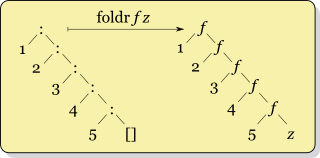
\includegraphics{Right-fold-transformation}
  \end{center}
\end{frame}
%----------------------------------------------------------------------
\begin{frame}[fragile]
  \frametitle{Foldr in action}
  \begin{block}<+->{sum and product}
\begin{verbatim}
sum xs     = foldr (+) 0 xs
product xs = foldr (*) 1 xs
\end{verbatim}
  \end{block}
  \begin{block}<+->{more functions}
\begin{verbatim}
or      xs = undefined
and     xs = undefined
concat  xs = undefined

maximum (x:xs) = undefined
\end{verbatim}
  \end{block}
\end{frame}
%----------------------------------------------------------------------
\begin{frame}[fragile]
  \frametitle{Foldr puzzles}
  \begin{block}<+->{f1}
\begin{verbatim}
f1 xs = foldr (:) [] xs
\end{verbatim}
  \end{block}
  \begin{block}<+->{f2}
\begin{verbatim}
f2 xs ys = foldr (:) ys xs
\end{verbatim}
  \end{block}
  \begin{block}<+->{f3}
\begin{verbatim}
f3 xs = foldr snoc [] xs
  where snoc x ys = ys++[x]
\end{verbatim}
  \end{block}
  \begin{block}<+->{f4}
\begin{verbatim}
f4 f xs = foldr fc [] xs
  where fc x ys = f x:ys
\end{verbatim}
  \end{block}
\end{frame}
%----------------------------------------------------------------------
\begin{frame}
  \frametitle{Transforming functions}
  \framesubtitle{Useful operations on functions}
  \begin{itemize}
  \item partial application
  \item operator sections
  \item function composition
  \item anonymous functions aka lambda expressions
  \item eta conversion
  \end{itemize}
\end{frame}
%----------------------------------------------------------------------
\begin{frame}[fragile]
  \frametitle{Partial application}
\begin{verbatim}
take :: Int -> [a] -> [a]
take 5 :: [a] -> [a]

foldr :: (a -> b -> b) -> b -> [a] -> b
foldr (+) :: Int -> [Int] -> Int
foldr (+) 0 :: [Int] -> Int
\end{verbatim}
  \begin{itemize}
  \item Partial application $=$ function application with ``too few'' arguments
  \item Result is a function
  \item Can be used like any other function
  \end{itemize}
\end{frame}
%----------------------------------------------------------------------
\begin{frame}[fragile]
  \frametitle{Operator sections}
\begin{verbatim}
-- subtraction
(-) :: Int -> Int -> Int
-- subtract one
(- 1) :: Int -> Int
-- subtract from one
(1 -) :: Int -> Int

-- less than 0
(< 0) :: Int -> Bool
-- greater than 0
(0 >) :: Int -> Bool
\end{verbatim}
  can be done with every infix function
\end{frame}
%----------------------------------------------------------------------
\begin{frame}[fragile]
  \frametitle{Function composition}
  \begin{block}{Example}
    \begin{itemize}
    \item<+-> Remove spaces from string as in this
      example
\begin{verbatim}
removeSpaces "abc def \n ghi" == "abcdefghi"
\end{verbatim}
    \item<+-> In module \texttt{Data.Char}
\begin{verbatim}
isSpace :: Char -> Bool
\end{verbatim}
    \item<+-> yields definition
\begin{verbatim}
removeSpaces xs = filter (not . isSpace) xs
\end{verbatim}
    \item<+-> Operator ``\texttt{.}'' is function composition defined by
\begin{verbatim}
(f . g) x = f (g x)
\end{verbatim}
    \item<+-> What's the type of \texttt{(.)}?
    \item<+-> \texttt{(.) :: (b -> c) -> (a -> b) -> (a -> c)}
    \end{itemize}
  \end{block}
\end{frame}
%----------------------------------------------------------------------
\begin{frame}[fragile]
  \frametitle{Anonymous functions}
  \begin{itemize}
  \item<+-> Usual function definition
\begin{verbatim}
snoc x ys = ys++[x]
\end{verbatim}
  \item<+->
  Alternative: define \texttt{snoc} using an anonymous function aka
  \href{https://en.wikipedia.org/wiki/Anonymous_function}{lambda
    expression} 
\begin{verbatim}
snoc = \ x ys -> ys++[x]
\end{verbatim}
  Nowadays, the Unicode lambda can also be used
\item<+->
  Often for function used in one place as in
\begin{verbatim}
f3 xs = foldr snoc [] xs
  where snoc x ys = ys++[x]
\end{verbatim}
\item<+-> Equivalently replace \texttt{snoc} by its definition
\begin{verbatim}
f3' xs = foldr (\ x ys -> ys++[x]) [] xs
\end{verbatim}
\item<+-> Shorten more using partial application
\begin{verbatim}
f3'' xs = foldr (\ x -> (++[x])) [] xs
\end{verbatim}
\end{itemize}
\end{frame}
%----------------------------------------------------------------------
\begin{frame}[fragile]
  \frametitle{Eta conversion}
  \begin{enumerate}
  \item A number of definitions have the form
\begin{verbatim}
f x = g x
\end{verbatim}
    where \texttt{x} does not occur in \texttt{g}
  \item 
    In such cases, the formal parameter \texttt{x} is redundant:
\begin{verbatim}
f = g
\end{verbatim}
    is an equivalent definition.
  \item The transformation from (1) to (2) is called \textbf{eta reduction}.\footnote{Reverse transformation: \textbf{eta expansion}; both directions: \textbf{eta conversion}}
  \item The typing of an eta-reduced definition is more restricted.
\end{enumerate}
\end{frame}
%----------------------------------------------------------------------
\begin{frame}[fragile]
  \frametitle{Examples for eta-reduced definitions}
\begin{verbatim}
sum = foldr (+) 0
product = foldr (*) 1
or = foldr (||) False
and = foldr (&&) True
concat = foldr (++) []
removeSpaces = filter (not . isSpace)
\end{verbatim}
\end{frame}
%----------------------------------------------------------------------
\begin{frame}[fragile]
  \frametitle{Exercises}
\begin{verbatim}
takeLine :: String -> String
-- takeLine "abc\ndef\nghi\n" == "abc"

takeWhile' :: (a -> Bool) -> [a] -> [a]
dropWhile' :: (a -> Bool) -> [a] -> [a]
\end{verbatim}
\end{frame}
%----------------------------------------------------------------------
\begin{frame}[fragile]
  \frametitle{Exercises}
\begin{verbatim}
lines :: String -> [String]
-- lines "abc\ndef\nghi\n" == ["abc", "def", "ghi"]

segments' :: (a -> Bool) -> [a] -> [[a]]

words :: String -> [String]
-- words "abc def  ghi" == ["abc","def","ghi"]
\end{verbatim}
\end{frame}
%----------------------------------------------------------------------
\begin{frame}[fragile]
  \frametitle{Exercises}
  Define a function that counts how many times words occur in a text and displays each word with its count.
\begin{verbatim}
wordCounts :: String -> [String]
\end{verbatim}
  Example use
\begin{verbatim}
*Main> putStr (wordCounts "hello clouds\nhello sky")
clouds: 1
hello: 2
sky: 1
\end{verbatim}
\end{frame}
%----------------------------------------------------------------------
\begin{frame}
  \frametitle{Wrapup}
  \begin{alertblock}{Higher-order functions}
  \begin{itemize}
  \item take functions as parameters,
  \item often have polymorphic types,
  % \item Haskell prefers curried function types.
  \item abstract common patterns (map, filter, foldr),
  \item enable powerful programming techniques (partial application, operator sections, function composition, anonymous functions, eta conversion).
  \end{itemize}
  \end{alertblock}
\end{frame}

% \begin{frame}
%   \frametitle{Break Time --- Questions?}
%   \begin{center}
%     \tikz{\node[scale=15] at (0,0){?};}
%   \end{center}
% \end{frame}


\end{document}

%%% Local Variables: 
%%% mode: latex
%%% TeX-master: t
%%% End: 
